% Didactic overview of the intrusive reduced references.
% Rows 1--3 explain the offline state construction; rows 4--5 summarize the
% three online operating modes and their common constitutive interface.
\definecolor{hpromblue}{RGB}{0,105,210}
\begin{tikzpicture}[x=1cm,y=1cm,font=\small,
  panel/.style={draw=black!55,rounded corners=2pt,line width=.55pt,fill=white},
  card/.style={draw=black!35,rounded corners=1.5pt,line width=.45pt,fill=white},
  flow/.style={-{Latex[length=2mm]},draw=blue!45!black,line width=.8pt},
  flowline/.style={draw=blue!45!black,line width=.8pt},
  secondaryflow/.style={-{Latex[length=1.7mm]},draw=black!55,line width=.65pt},
  stage/.style={circle,draw=black!60,fill=black!72,text=white,
                font=\bfseries\footnotesize,minimum size=5.2mm,inner sep=0pt},
  snapshot/.style={draw=green!45!black,fill=green!23,line width=.55pt},
  affineblock/.style={draw=hpromblue!85!black,fill=hpromblue!24,line width=.65pt},
  basisprimary/.style={draw=blue!65!black,fill=blue!14,line width=.55pt},
  basissecondary/.style={draw=red!55!black,fill=red!14,line width=.55pt},
  statevector/.style={draw=green!45!black,fill=green!17,line width=.55pt},
  coordprimary/.style={draw=blue!65!black,fill=blue!8,rounded corners=1pt},
  coordsecondary/.style={draw=red!55!black,fill=red!8,rounded corners=1pt},
  neuron/.style={circle,draw=black!45,fill=white,minimum size=2.4mm,inner sep=0pt}
]
 \path[use as bounding box] (0,0) rectangle (16.2,21.2);

 % -----------------------------------------------------------------------
 % Row 1: generate microscopic displacement snapshots.
 \node[panel,minimum width=16.10cm,minimum height=3.05cm,anchor=south west]
   (generation) at (0,18.02) {};
 \node[stage] at (.36,20.67) {1};
 \node[font=\small\bfseries,anchor=west] at (.74,20.67)
   {RVE snapshot generation};

 \node[inner sep=0pt] (sampling) at (1.42,19.32)
   {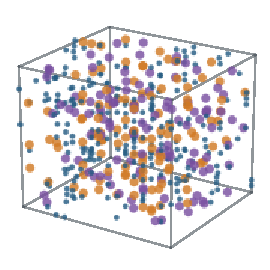
\includegraphics[width=1.58cm]{sampling_material_a_overview.pdf}};
 \node[font=\scriptsize,text=black!62] at (1.42,18.33)
   {sampled strains $\ee^s$};
 \node[inner sep=0pt] (rvesolve) at (4.30,19.32)
   {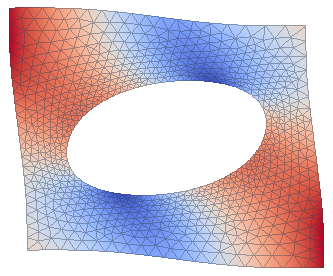
\includegraphics[width=2.10cm]{rve_deformed_overview.pdf}};
 \node[font=\scriptsize,align=center] at (4.30,18.33)
   {periodic FOM solve};
 \draw[flow] (sampling.east)--(rvesolve.west);
 \node[font=\tiny,text=black!58] at (2.73,19.57) {apply $\ee^s$};

 % Every column is a centered HDM state with the same dimension N.
 \node[font=\tiny,text=black!58] at (8.15,20.25)
   {$\widehat{\bm u}^{\,s}:=\bm u^s-\bm u_{\rm ref}$};
 \foreach \xx/\lab in {7.05/{\widehat{\bm u}^{\,1}},
                         7.92/{\widehat{\bm u}^{\,2}}} {
   \draw[snapshot] ({\xx-.21},18.64) rectangle ({\xx+.21},20.04);
   \node[font=\tiny] at (\xx,19.34) {$\lab$};
 }
\draw[snapshot] (9.29,18.64) rectangle (9.71,20.04);
\node[font=\tiny] at (9.50,19.34)
  {\scalebox{0.76}{$\scriptscriptstyle\widehat{\bm u}^{\,N_s}$}};
 \node[font=\normalsize] at (8.72,19.34) {$\cdots$};
 \node[font=\scriptsize,align=center] at (8.15,18.33)
   {centered displacement snapshots};
 \draw[flow] (rvesolve.east)--(6.72,19.32);

 \node[font=\scriptsize] at (13.30,20.25) {snapshot matrix};
 % Four vector-width units suggest the assembly of several N-vectors.
 \node[snapshot,minimum width=1.68cm,minimum height=1.40cm]
   (snapmatrix) at (13.30,19.34) {$\bm S_{\rm snap}$};
 \node[font=\tiny,text=black!58] at (13.30,18.46) {$N\times N_s$};
 \draw[flow] (9.84,19.32)--(snapmatrix.west);

 % -----------------------------------------------------------------------
 % Row 2: the same snapshot matrix generates either basis organization.
 \node[panel,minimum width=16.10cm,minimum height=3.10cm,anchor=south west,
       fill=black!1] (bases) at (0,14.60) {};
 \node[stage] at (.36,17.30) {2};
 \node[font=\small\bfseries,anchor=west] at (.74,17.30)
   {From the snapshot matrix to the reduced bases};

 % The matrix assembled in row 1 feeds both basis constructions directly.
 \node[card,minimum width=5.55cm,minimum height=2.02cm] (affinebasis)
   at (4.03,15.67) {};
 \node[font=\scriptsize] at (4.03,16.42) {affine basis};
 \draw[affineblock] (3.47,14.88) rectangle (4.59,16.28);
 \node[font=\scriptsize] at (4.03,15.58) {$\bm V_{\rm tra}$};
 \node[font=\tiny,text=black!58] at (4.03,14.75)
   {$N\times n_{\rm tra}$};

 \node[card,minimum width=5.55cm,minimum height=2.02cm] (splitbasis)
   at (12.08,15.67) {};
 \node[font=\scriptsize] at (12.08,16.42) {partitioned basis};
 \draw[basisprimary] (11.52,14.88) rectangle (11.94,16.28);
 \draw[basissecondary] (11.94,14.88) rectangle (12.64,16.28);
 \node[font=\scriptsize] at (11.73,15.58) {$\bm V$};
 \node[font=\scriptsize] at (12.29,15.58) {$\overline{\bm V}$};
 \node[font=\tiny,text=black!58] at (12.08,14.75)
   {$N\times(n+\bar n)$};

 % The route exits to the right, descends beside the panels, and becomes a
 % horizontal bus.  The two downward arrows then identify the alternatives.
 \coordinate (basisbusleft) at (4.03,16.98);
 \coordinate (basisbusright) at (15.82,16.98);
 \draw[flowline,rounded corners=2pt]
   (snapmatrix.east)--(15.82,19.34)--(basisbusright)--(basisbusleft);
 \draw[flow] (4.03,16.98)--(affinebasis.north);
 \draw[flow] (12.08,16.98)--(splitbasis.north);

 % -----------------------------------------------------------------------
 % Row 3: dimensional block diagrams for the two state representations.
 \node[panel,minimum width=16.10cm,minimum height=4.55cm,anchor=south west]
   (representations) at (0,9.72) {};
 \node[stage] at (.36,13.87) {3};
 \node[font=\small\bfseries,anchor=west] at (.74,13.87)
   {Two reduced representations of the microscopic state};
 \node[font=\scriptsize,fill=white,inner sep=1.5pt] at (8.05,13.46)
   {$\widehat{\widetilde{\bm u}}:=
     \widetilde{\bm u}-\bm u_{\rm ref}$};

 \node[card,fill=hpromblue!2,minimum width=7.45cm,minimum height=3.24cm]
   (affinestate) at (4.03,11.48) {};
 \node[font=\scriptsize\bfseries,text=hpromblue!82!black] at (4.03,12.80)
   {Affine HPROM state};
 \node[font=\scriptsize] at (4.03,12.44)
   {$\widehat{\widetilde{\bm u}}=
     \bm V_{\rm tra}\qq_{\rm tra}$};
 \draw[statevector] (1.45,10.60) rectangle (1.87,12.00);
 \node[font=\tiny] at (1.66,11.31)
   {$\widehat{\widetilde{\bm u}}$};
 \node[font=\scriptsize] at (2.18,11.31) {$=$};
 % n_tra = n + nbar is encoded by the total block width.
 \draw[affineblock] (2.50,10.60) rectangle (3.62,12.00);
 \node[font=\scriptsize] at (3.06,11.31) {$\bm V_{\rm tra}$};
 \node[font=\scriptsize] at (3.88,11.31) {$\times$};
 \draw[affineblock,rounded corners=1pt]
   (4.16,10.75) rectangle (4.58,11.87);
 \node[font=\tiny] at (4.37,11.31) {$\qq_{\rm tra}$};
 \node[font=\tiny] at (1.66,10.43) {$N$};
 \node[font=\tiny] at (3.06,10.34) {$N\times n_{\rm tra}$};
 \node[font=\tiny] at (4.37,10.50) {$n_{\rm tra}$};
 \node[font=\scriptsize,align=center] at (4.03,10.06)
   {$n_{\rm tra}$ independent coordinates};

 \node[card,fill=teal!1,minimum width=7.45cm,minimum height=3.24cm]
   (nonlinearstate) at (12.08,11.48) {};
 \node[font=\scriptsize\bfseries,text=teal!65!black] at (12.08,12.80)
   {HPROM--ANN nonlinear state};
 \node[font=\scriptsize] at (12.08,12.44)
   {$\widehat{\widetilde{\bm u}}=
     \bm V\qq+\overline{\bm V}\mathcal N(\qq)$};
 \draw[statevector] (8.45,10.60) rectangle (8.87,12.00);
 \node[font=\tiny] at (8.66,11.31)
   {$\widehat{\widetilde{\bm u}}$};
 \node[font=\scriptsize] at (9.10,11.31) {$=$};
 % The blue and red basis widths sum to the width of V_tra above.
 \draw[basisprimary] (9.42,10.60) rectangle (9.84,12.00);
 \node[font=\tiny] at (9.63,11.31) {$\bm V$};
 \draw[coordprimary] (10.03,11.10) rectangle (10.45,11.52);
 \node[font=\tiny] at (10.24,11.31) {$\qq$};
 \node[font=\scriptsize] at (10.66,11.31) {$+$};
 \draw[basissecondary] (10.91,10.60) rectangle (11.61,12.00);
 \node[font=\tiny] at (11.26,11.31) {$\overline{\bm V}$};
 \node[font=\scriptsize] at (11.84,11.31) {$\times$};
 \node[font=\tiny] at (8.66,10.43) {$N$};
 \node[font=\tiny] at (9.63,10.43) {$N\times n$};
 \node[font=\tiny] at (10.24,10.88) {$n$};
 \node[font=\tiny] at (11.26,10.43) {$N\times\bar n$};

 % The network box is the factor N(q); its output has the complementary
 % height so that q and qbar together match q_tra on the left.
 \draw[draw=black!25,rounded corners=1.5pt,fill=white]
   (12.08,10.55) rectangle (15.45,12.03);
 \node[font=\tiny,text=teal!65!black,fill=teal!1,inner sep=1pt]
   at (13.76,12.13)
   {$\mathcal N(\qq)$};
 \draw[coordprimary] (12.24,11.10) rectangle (12.66,11.52);
 \node[font=\tiny] at (12.45,11.31) {$\qq$};
 \foreach \j/\yy in {1/10.90,2/11.31,3/11.72}
   \node[neuron] (nh\j) at (13.23,\yy) {};
 \foreach \j/\yy in {1/10.90,2/11.31,3/11.72}
   \node[neuron] (nk\j) at (13.87,\yy) {};
 \draw[coordsecondary] (14.79,10.96) rectangle (15.21,11.66);
 \node[font=\tiny] (netout) at (15.00,11.31)
   {$\overline{\qq}$};
 \foreach \j in {1,...,3} {
   \draw[draw=black!38,line width=.35pt] (12.66,11.31)--(nh\j.west);
   \draw[draw=black!38,line width=.35pt] (nk\j.east)--(14.79,11.31);
   \foreach \k in {1,...,3}
     \draw[draw=black!28,line width=.28pt] (nh\j.east)--(nk\k.west);
 }
 \node[font=\tiny,text=black!58] at (12.45,10.76) {$n$};
 \node[font=\tiny,text=black!58] at (15.00,10.72) {$\bar n$};
 \node[font=\scriptsize] at (12.08,10.06)
   {only $\qq$ is solved independently};

 % -----------------------------------------------------------------------
 % Row 4: online use of the state representations and sparse rules.
 \node[panel,minimum width=16.10cm,minimum height=6.00cm,anchor=south west]
   (routes) at (0,3.35) {};
 \node[stage] at (.36,8.95) {4};
 \node[font=\small\bfseries,anchor=west] at (.74,8.95)
   {Three online routes};
 \node[card,fill=orange!3,minimum width=4.25cm,minimum height=.58cm]
   (commoninput) at (8.05,8.95)
   {\scriptsize prescribed macroscopic strain $\ee$};

 \node[panel,fill=hpromblue!2,minimum width=4.72cm,minimum height=4.55cm]
   (hpromcol) at (2.67,5.83) {};
 \node[font=\small\bfseries,text=hpromblue!82!black] at (2.67,7.87) {HPROM};
 \node[card,minimum width=3.48cm,minimum height=.55cm] (hroute)
   at (2.67,7.32) {\scriptsize affine reconstruction};
 \node[inner sep=0pt] (hsupport) at (2.67,6.09)
   {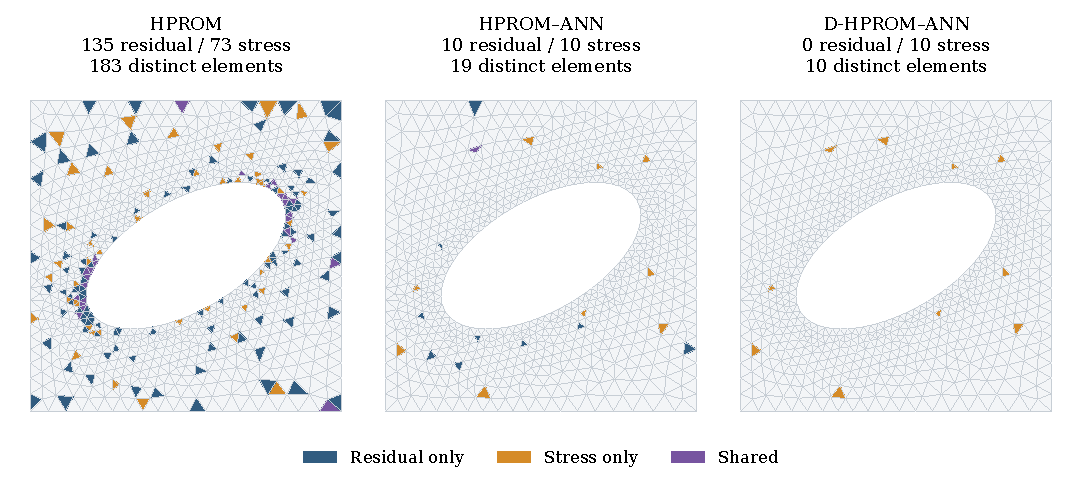
\includegraphics[width=1.75cm,trim=10bp 34bp 348bp 48bp,clip]
      {reduced_supports.pdf}};
 \node[font=\scriptsize,align=center] (hrules) at (2.67,4.96)
   {fixed residual/stress rules\\[-.08em]
    \textcolor{black!58}{$\approx4\%$ of FOM elements}};
 \node[card,minimum width=3.48cm,minimum height=.88cm]
   (hsolve) at (2.67,4.10) {};
 % The residual-vector heights mirror the solved coordinate dimensions.
 \draw[affineblock,rounded corners=.7pt]
   (1.16,3.83) rectangle (1.48,4.43);
 \node[font=\tiny] at (1.32,4.13)
   {$\scriptscriptstyle\bm r_h$};
 \node[font=\tiny,text=black!58] at (1.32,3.76) {$n_{\rm tra}$};
 \node[font=\scriptsize,align=center] at (2.92,4.12)
   {projected equilibrium\\[-.08em]
    $\bm r_h(\qq_{\rm tra};\ee)=\bm0$};

 \node[panel,fill=teal!2,minimum width=4.72cm,minimum height=4.55cm]
   (hpanncol) at (8.05,5.83) {};
 \node[font=\small\bfseries,text=teal!65!black] at (8.05,7.87)
   {HPROM--ANN};
 \node[card,minimum width=3.48cm,minimum height=.55cm] (haroute)
   at (8.05,7.32) {\scriptsize nonlinear decoder};
 \node[inner sep=0pt] (hasupport) at (8.05,6.09)
   {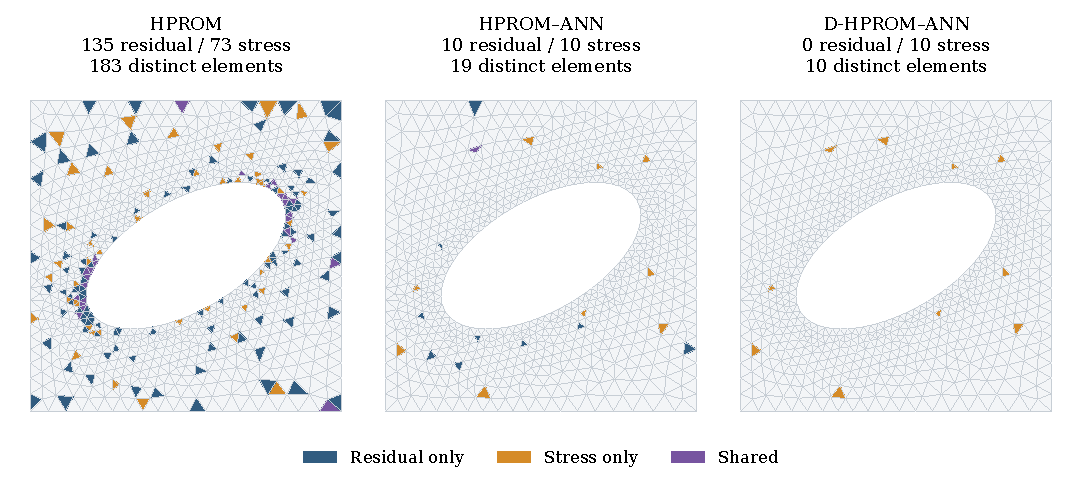
\includegraphics[width=1.75cm,trim=180bp 34bp 175bp 48bp,clip]
      {reduced_supports.pdf}};
 \node[font=\scriptsize,align=center] (harules) at (8.05,4.96)
   {adaptive residual/stress rules\\[-.08em]
    \textcolor{black!58}{$\approx0.4\%$ of FOM elements}};
 \node[card,minimum width=3.48cm,minimum height=.88cm]
   (hasolve) at (8.05,4.10) {};
 \draw[coordprimary,line width=.65pt,rounded corners=.7pt]
   (6.54,3.96) rectangle (6.86,4.30);
 \node[font=\tiny] at (6.70,4.13)
   {$\scriptscriptstyle\bm r_h$};
 \node[font=\tiny,text=black!58] at (6.70,3.81) {$n$};
 \node[font=\scriptsize,align=center] at (8.30,4.12)
   {projected equilibrium\\[-.08em]
    $\bm r_h(\qq;\ee)=\bm0$};

 \node[panel,fill=violet!2,minimum width=4.72cm,minimum height=4.55cm]
   (dhpanncol) at (13.43,5.83) {};
 \node[font=\small\bfseries,text=violet!70!black] at (13.43,7.87)
   {D-HPROM--ANN};
 \node[card,minimum width=3.48cm,minimum height=.55cm] (droute)
   at (13.43,7.32) {\scriptsize direct decoder, $\bm\xi=\ee$};
 \node[inner sep=0pt] (dsupport) at (13.43,6.09)
   {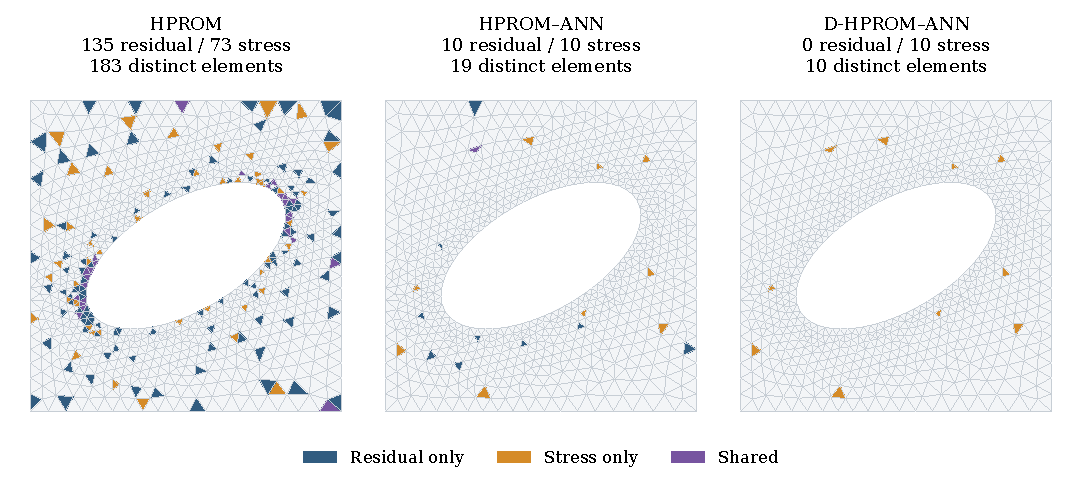
\includegraphics[width=1.75cm,trim=355bp 34bp 5bp 48bp,clip]
      {reduced_supports.pdf}};
 \node[font=\scriptsize,align=center] (drules) at (13.43,4.96)
   {adaptive stress rule\\[-.08em]
    \textcolor{black!58}{$\approx0.2\%$ of FOM elements}};
 \node[card,minimum width=3.48cm,minimum height=.88cm,align=center]
   (dsolve) at (13.43,4.10)
   {\scriptsize one-pass state evaluation\\[-.08em]
    \scriptsize $\ee\longmapsto\widetilde{\bm u}_{D}(\ee)$};

 \draw[flowline] (commoninput.south)--(8.05,8.42);
 \draw[flowline] (2.67,8.42)--(13.43,8.42);
 % The common loading enters through the center of each route frame.
 \draw[flow] (2.67,8.42)--(hpromcol.north);
 \draw[flow] (8.05,8.42)--(hpanncol.north);
 \draw[flow] (13.43,8.42)--(dhpanncol.north);
 \foreach \a/\b/\c/\d in {hroute/hsupport/hrules/hsolve,
                             haroute/hasupport/harules/hasolve,
                             droute/dsupport/drules/dsolve} {
   \draw[secondaryflow] (\a.south)--(\b.north);
   \draw[secondaryflow] (\c.south)--(\d.north);
 }

 % -----------------------------------------------------------------------
 % Row 5: common microscopic output interface.
 \node[panel,minimum width=16.10cm,minimum height=2.96cm,anchor=south west,
       fill=green!1] (outputpanel) at (0,.05) {};
 \node[stage] at (.36,2.60) {5};
 \node[font=\small\bfseries,anchor=west] at (.74,2.60)
   {Common constitutive output};
 \node[card,minimum width=4.05cm,minimum height=.82cm,align=center]
   (microlaw) at (3.10,1.18)
   {\scriptsize output cubature\\[-.05em]
    \scriptsize $\bm P_h=
      |Y|^{-1}\!\displaystyle\sum_{e\in\mathcal Z_s}v_e\bm P_e$};
 \node[card,fill=green!3,minimum width=3.15cm,minimum height=.82cm,align=center]
   (stressout) at (8.15,1.18)
   {\scriptsize work-conjugate stress $\ssv_h$};
 \node[card,fill=blue!3,minimum width=3.15cm,minimum height=.82cm,align=center]
   (tangentout) at (12.90,1.18)
   {\scriptsize consistent tangent $\bm D_h$};
 \draw[flow] (microlaw.east)--(stressout.west);
 \draw[flow] (stressout.east)--(tangentout.west);
 \draw[flowline] (hsolve.south)--(2.67,3.18);
 \draw[flowline] (hasolve.south)--(8.05,3.18);
 \draw[flowline] (dsolve.south)--(13.43,3.18);
 \draw[flowline] (2.67,3.18)--(13.43,3.18);
 % Enter below the heading so that the common route does not cross its text.
 \draw[flow,rounded corners=2pt]
   (8.05,3.18)--(8.05,2.10)--(3.10,2.10)--(microlaw.north);
 \node[font=\tiny,text=black!58] at (8.05,.24)
   {same FE$^2$ interface; different state, integration, and equilibrium approximations};
\end{tikzpicture}
